\documentclass[10pt, oneside]{article}

\usepackage{geometry}
\geometry{a4paper}
\usepackage[utf8]{inputenc}
\usepackage{graphicx}
\usepackage{amssymb}
\usepackage{authblk}
\usepackage{multicol}
\usepackage{rotating}
\usepackage{capt-of}
\usepackage{hyperref}	%autoref
\usepackage{amsmath}	%equation*
\usepackage{array}
\newenvironment{Figure}
    {\par\medskip\noindent\minipage{\linewidth}}
    {\endminipage\par\medskip}

\usepackage{lipsum}
\usepackage{parskip}    % spacing between paragraphs instead of indention  


\title{Multi-agent Systems Project Report: \\
    Traffic Simulation based on Real-Time Information}

\author[]{Konstantin Kloster}
\author[]{Oliver Berg}
\affil[1]{Technical University Kaiserslautern}

\date{\today}


\begin{document}
\maketitle

% \begin{multicols}{2}


\begin{abstract}
    % when doc finished, summarize task+approach+results
    \lipsum[1]
    \lipsum[2]
\end{abstract}

\tableofcontents

\newpage
\section{Introduction}
    \lipsum[1]       % CHECK; paraphrasing task description, foreshadowing setup + analysis, explaining sections
\newpage
\section{Related Work}\label{sec:relatedWork}

Simulating development of traffic is a well-traversed research topic regarding scheduling and network traversal simulation problems.
Throughout application, dedicated simulators have been applied frequently and early-on like the popular "Multi-agent Transport Simulator" (MATSim) \cite{sezen2003modeling} or "Repast Simphony" \cite{zargayouna2013agent} alongside dedicated extensions like the Symphony-based "SM4T Simnulator" \cite{ksontini2016building}.
Such applications provide advantages like automated timetables for public transport, advanced types of travelling agent and unified logging formats for simulation runs.
Resorting to holistic solutions like the above mentioned is especially useful for non-technological research regarding behavioral analysis or city planning \cite{brakewood2018literature}. If the multi-agent system aspects are predominant though (as is the case in this work), adapting similar implementation structures whilst doing the actual agent implementation work (done here) proves beneficial.

In contrast to fully incorporated applications, some approaches in literature already shift focus towards surrounding aspects surrounding of traffic simulation, like focusing on the distributing simulation \cite{mastio2015towards}.

As of \cite{mastio2015towards}, which depicts the simplest yet most fundamental approach to general network traversal, it utilizes a basic graph structure with vertices (also called "nodes") as intersection points and edges (also called "links") connecting these intersections. Agents are assigned a path over a fixed set of vertices as the shortest path over weighted edges. Path updates may occur only upon arrival at a given vertex when the agent then queries for a possible updated path.
The travel time $t$ on an edge depends on the number of agents currently on the edge in question. Calculating this $t$ can be done based on different kinds of functions modelling e.g. a certain free-flow capacity where for a given $n$ number of vehicles the weight ($t$) of an edge will not be impacted and only after reaching a certain threshold number $n_{\text{thresh}}$ the weight will increase to depict a slower movement (to a degree of $\alpha$) of traffic along said edge; exemplary formulas can, for example, be found in \cite{mastio2015towards} or \cite{ksontini2016building}.

To this agent-centric travel choice procedure, a literature review as is being depicted in the transport review of \cite{brakewood2018literature} adds a theoretical framework of traveler agent's perspective concerning travel- and mode choice as well as choices regarding route, boarding and departure. Incorporating this thinking, one ends up with a tight path-choosing procedure across multiple channels which theoretically boils down to the simple procedure of the previously mentioned formulas adapted to modes, routes and fixed schedules.
As this framework is a theoretical methodology at heart, the practical implementation aspect of this formal procedure raises multiple performance and architectural issues which without utilizing afore-mentioned well-established holistic framework solutions is expected to introduce bottlenecks.

As proposed by \cite{zargayouna2013agent}, agents adhere to a specific simulation workflow where they continuously query for updates regarding path choice whenever reaching nodes of the underlying network. Opposing the precise setup depicted here and utilizing in addition the thinking of \cite{mastio2015towards}, no precise time-step-based approach of procedurally checking all agents for their position but rather an event-based truly (distributed) multi-agent approach is implemented where agents query after complete time lapses instead of single short global time intervals. 

The visualization procedure of a given simulation then needs to adhere to the time lapse nature of the event logs, which not necessarily adheres well to standards defined by holistic framework solutions (like used in \cite{zargayouna2013agent}\cite{ksontini2016building}). As visualization is a side-aspect of most MAS-focused implementations (see \cite{mastio2015towards}), this is generally speaking seen as an added bonus for both debugging and reporting purposes.

Regarding performance metrics of a traffic simulation, metrics like use-of-transit, satisfaction and travelling-time are frequently proposed (\cite{brakewood2018literature}). With the use of dedicated car- and planner-agents (alongside \cite{zargayouna2013agent}) and the omittance of public transport time-table-based scheduling / availability-based carsharing, this leaves travelling-time as well as deviation from planning to execution performance as major indicators for performance.
In addition to this, subjective monitoring of network behavior may enhance the result (\cite{brakewood2018literature}, \cite{zargayouna2013agent}).
     % TODO: (NXT) go through provided sources (4) as well as (generally) connected material
\newpage
\section{MAS Traffic Simulator Backend}\label{sec:backend}

\lipsum[3]

% Car Agent types be LOCAL, SEMI_LOCAL, GLOBAL
% respective type of information available / being queried from planner-agent

% Public transit is due to complexity of formal representation of timetables not done.     % Python MAS setup, graph-type, agent-type, communication setup
\newpage
\section{Web-based Simulation Frontend}\label{sec:frontend}

Following the in \autoref{sec:backend} described MAS architecture, this section now presents the web-based frontend application visualizing a simulation run based on the persisted simulation run logging information and other provided miscellaneous resources. 


\subsection{Persisted Logging Information}

The frontend application reads graphs from json-files as well as a corpus of simulation-run logging files.


\subsubsection{Graphs}\label{subsubsec:graphs}

The network graph json-files are generated via the Python framework GraphX and then stored as json-files in the project folder. These are then being read from the MAS backend as well as the frontend-application. The file format can be seen in the example of figure below.

\begin{figure}[thp]
    \centering
    \lstset{language=json, frame=single, linewidth=11cm}
    \begin{tabular}{c}
        \begin{lstlisting}
{
    "directed": false,
    "graph": {
        "name": "A Testing Graph"
    },
    "links": [
        {"source": 0, "target": 1, "value":1},
        {"source": 1, "target": 0, "value":2}
    ],
    "multigraph": false,
    "nodes": [
        {"id": 0, "color": "purple", "size": 16},
        {"id": 1, "color": "green", "size": 9}
    ]
}
        \end{lstlisting}
    \end{tabular}
    \caption{Example of GraphX output format (JSON)}
    \label{fig:graphx}
\end{figure}

These graphs are being read form disc and parsed into program structures (backend) or exposed to an API (frontend, see \autoref{subsec:frontendArchitecture}).

They do however only depict the formal structure of the graph, which is all the backend needs to simulate agent paths. For a proper visualization of the graph on the 2D image plane, the web-frontend additionally utilizes some formal graph-drawing algorithms (see \autoref{subsec:d3}).


\subsubsection{Simulation-Logs}

The simulation logs are the actual output of the traffic simulator and come on a collection of multiple associated logs: 

\begin{itemize}
    \item \textit{[id]-[graphId]-carAgents.log}
    \item \textit{[id]-[graphId]-plannerAgent.log}
    \item \textit{[id]-[graphId]-events.log}
\end{itemize}

Each log is named by a unique id which is unique only across multiple sets of different logs but coherent across all associated logs. This allows to map each carAgents-log to its respective event-log and plannerAgent-log.
The graph-id is specified for each set of associated logs in order to map the utilized graph to the logs. Logs of a respective simulation run can only be visualized for the specified graph it was run on.

Each log-file has lines for any event occurring at a specified point in time (indicated with the line's initial timestamp-value) and multiple values separated with semicolons.

The \textbf{carAgents-log} holds lines structured with values of: \textit{timestamp} (ts), \textit{action} ("spawn" / "enter" / "reach" / "despawn"), \textit{agentID} and depending on the action some more attributes. It as such depicts the events thrown by car-agents and logged to reason about their timely execution.
Action-type "spawn" gets additional attributes \textit{spawnNode} and \textit{agentType} to specify where and which kind of (car-)agent was spawned. 
Action-type "enter" gets additional attributes \textit{linkEdgeFrom}, \textit{linkEdgeTo} and \textit{linkValue} to specify which edge the agent entered and at which speed he will traverse the link.
Action-type "reach" gets the additional attribute \textit{node} to declare which (final) node the agent has just reached.
Action-type "despawn" finally does not get additional attributes as this action only indicates to remove the agent from all later considerations.

The \textbf{plannerAgent-log} holds lines structured with values of: \textit{timestamp} (ts), \textit{action} ("init" / "update" / "reroute"), \textit{agentId}, \textit{routeNodes} and \textit{routeLinkValues}, where the both "routeNodes" and "routeLinkValues" are lists of ids / numbers respectively indicating graph edges and edge weights of paths. As such this log captures the path planning done by the planner-agent for car-agents on initialization, updating of path link weights when reaching vertices or rerouting with new vertices and edges all together.

The \textbf{events-log} holds lines structured with values of: \textit{timestamp} (ts), \textit{listOfEdges} and \textit{factor}, where the "listOfEdges" presents a list of nodes that identify links between them to be impacted in their weight / speed by the provided "factor".
As such, the events viable for the application include all types of events that impact a given set of linked concerning travelling speed. This type of event was identified as being the most general one whilst having a major impact in route planning and provides intuitive real-world counterparts (e.g. break-down of a node slows down all traffic to that node, break down in a rode is a single link being impacted, new road means a single link becomes faster to use).


\subsection{Frontend Architecture}\label{subsec:frontendArchitecture}

The overall frontend application's architecture is based on a traditional Model-View-Controller setup implemented in NodeJS. The webserver is setup to listen to port 3000 and receive http requests to then respond with the corresponding page content.

Internally, an API plays the role of the controller-component connecting the view-layer to the model. This interface is being utilized primarily to expose local file data to the end-user via a unified interface, preemptively resolving possible difficulties connecting the frontend application to the backend result or later adding further functionality based on said data. It is used to return json-formated data on graphs, logs and other miscellaneous internal status information.

The API primarily talks to the \textit{masSimulatorConnection} which reads, formats and persists logging and graph information as it is being setup in the web-UI.
Please note that as such the web-page is not quite capable to handle multi-user when being deployed, but rather a single user entity.

Through the dedicated intermediate API layer, access control for resources as requested by the end-user application would be both possible and straight -forward to implement later on if needed.


\subsection{User Interface Experience}

The exposed User Interface depicts a web-page written in plain HTML5, CSS3 and JavaScript with the help of common libraries such as \textit{jQuery} and \textit{Bootstrap} for simple best-practice setup in addition to \textit{toastr} for notifications (see \autoref{fig:web-ui-init}).

\begin{figure}
    \centering
    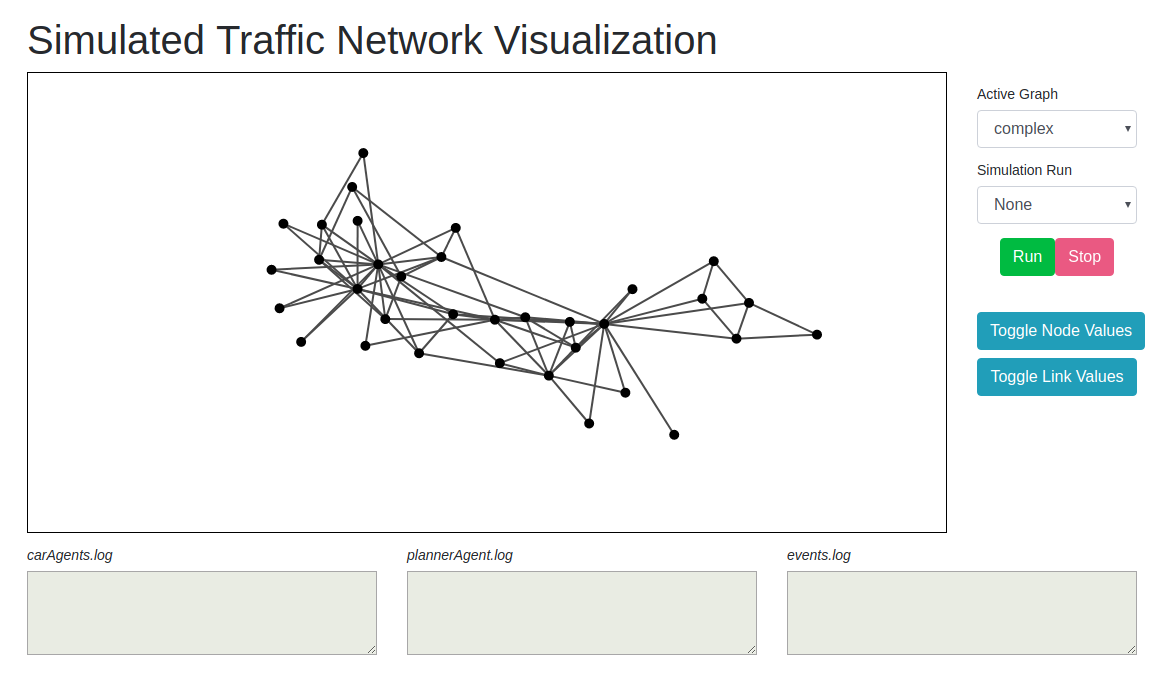
\includegraphics[width=0.9\textwidth]{images/web-ui-init.png}
    \caption{Web-UI upon initial loading of the page}
    \label{fig:web-ui-init}
\end{figure}

For canvas-based visualization and especially animation, the visualization library \textit{D3.js} was utilized (more on that in \autoref{subsec:d3}).

The navigation flow adheres to basic top-to-bottom / left-to-right principle: The network graph is displayed in the canvas to the upper left, from which the selections take place to its right via selection panels for graph and simulation run. Controls regarding run visualization are positioned directly under the run selection with appropriate colors for starting and stopping. General non-intrusive display options (turning on Node-ID / Link-ID displays) are presented in more neutral blue color and positioned below the other primary controls.

Below the basic visualization panel, textareas are used to display retrieved current-run logs (conforming to the conventions established in \autoref{subsubsec:graphs}). These serve the purpose to more intuitively display the information available from the simulation for visualization, as well as give instant feedback to selections made regarding the simulation run. Selections made regarding graph network immediately prompt a redrawing of the new network. All selections and button presses yield immediate visual feedback (via onchange-events).

To ease the usage of the frontend navigation elements, they are en-/disabled based on the state of the application. As such, only simulation runs belonging to the currently active (drawn) graph are enabled for selection in the second select, the run-button only gets enabled with a drawn graph and selected run and the stop-button is disabled as long as no simulation is running.


\subsection{Web-based Animations with D3}\label{subsec:d3}

The underlying animation and visual display of graph elements are being done via the visualization library \textit{D3.js} \cite{bostock2012d3}.
Generally speaking, it is based on the assumption that instead of separate independent graphical operations, D3 takes arrays of objects and manipulates (svg-) objects based on this set of provided data-points. Through procedure, the visualization of an array of vertices and edges becomes much more intuitive as well as computationally feasible.

In \autoref{fig:web-ui-running}, you see a running simulation visualization as it is being projected on the drawn network graph.

\begin{figure}
    \centering
    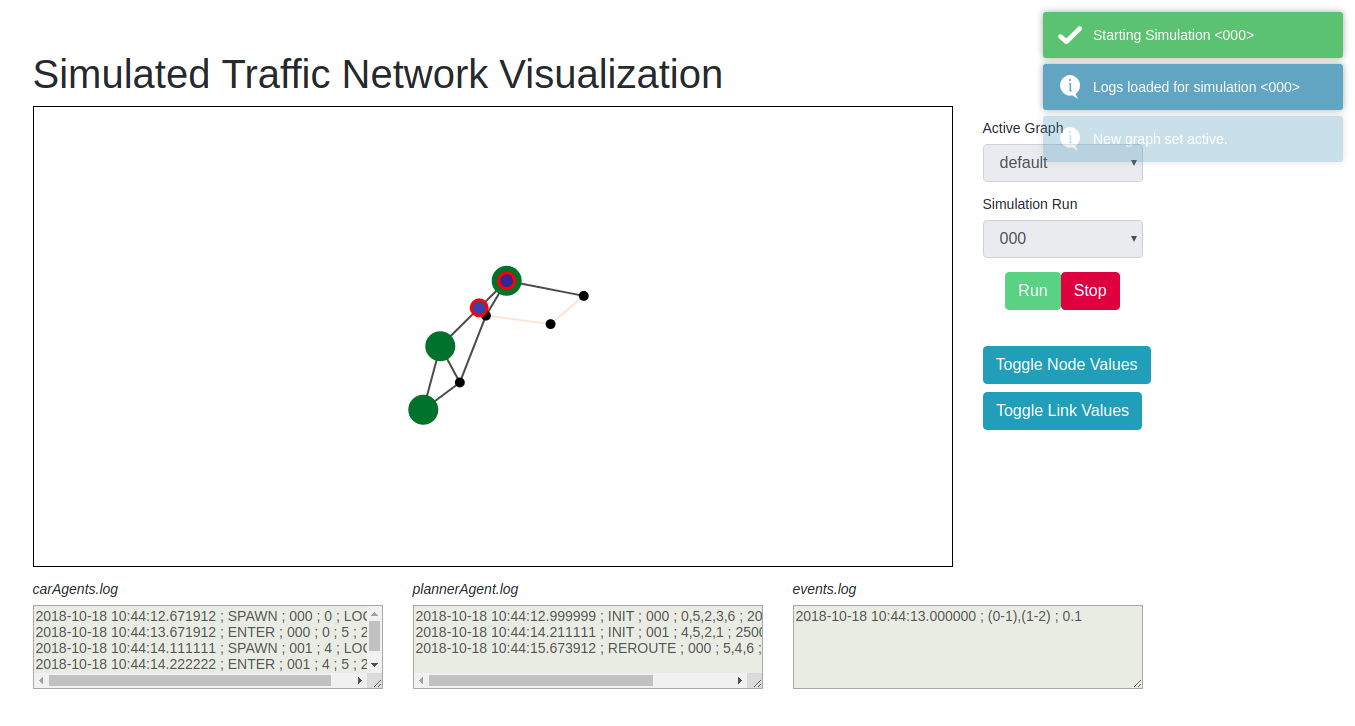
\includegraphics[width=0.9\textwidth]{images/web-ui-running.png}
    \caption{Web-UI with running visualization}
    \label{fig:web-ui-running}
\end{figure}

The graph-drawing utilizes D3's dynamic visualization procedure to create a force-directed layout of the theoretical network description. Throughout D3's iteration, fixed positional and directional values are being applied, making the drawing process - though being dynamic - a deterministic process, thus drawing the same graph visualization of a given graph every time it is being called upon to be drawn on the canvases 2D plane.
Animations are created by transform-operations on svg-elements on the canvases.

Regarding concrete visualization of simulation-run events:
Agents are drawn as circles of similar shape compared to nodes (as they are initially spawned on top of nodes of the network, thus maintaining similarity is intuitive) with borders indicating the type of (car-)agent displayed ("local" / "semi-local" / "global") and body colors ranging in the randomly interpolated blue spectrum.
Upon path-scheduling by the planner-agent, the nodes of the identified path are briefly highlighted (increased in shape) in the same color as the agent the path was identified for. Updating paths only based on new link-values without rerouting does not prompt a visual feedback, while rerouting actions prompt similar highlighting as done uponm initialization, but in the respectively interpolated green color spectrum for all nodes included in the new path.

The overall setup of animations is timestamp-based, as the globally initial (smallest) timestep in the car-agents-log is identified and set as \textit{time-0}, to then set timeouts for all other log entries based on the difference in timestamp values to this zero-time.
    % TODO: File-reading (graphs, logs), NodeJS architecture, D3, graph-drawing, UI
\newpage
\section{Agent Performance Analysis}\label{sec:performanceAnalysis}

Having presented MAS backend traffic simulation and frontend visualization procedures in \autoref{sec:backend} and \autoref{sec:frontend} respectively, we now add evaluation procedure and its implementation as well as resulting performance metrics.


\subsection{Evaluation Procedure}

There are different types of agents (of \textit{local} or \textit{global} nature) with randomly engaged origin and destination nodes as well as random events influencing the state of the network. Agents move along edges and thus reduce the speed of other agents proceeding to traverse said edge.

With ouputs of the underlying simulation on carAgents-, planner- and events-log together with the graph-file, all performance metrics can be retrieved from these information:
\begin{itemize}
    \item The planner-log allows to compute \textbf{expected travelling time} from the initiated path for an agent with the weights of the edges as depicted in the graph-file
    \item From 'spawn'- and 'reach'-events in the carAgents-log, the \textbf{actual travelling time} can be computed. Note that the actual travelling time may never be larger than the expected travelling time, as events in the network never speed-up edge traversal and traversal time gets impacted only negatively by other car-agents.
    \item Subtracting expected from actual travelling time yields the agent's \textbf{travelling time discrapency}, which depicts one of the major performance number
    \item Also note that the carAgent-log's 'spawn'-event holds information regarding the \textbf{type of car-agent} spawned. Travelling time information is persisted and compared with regards to the respective car-agent type as well.
    \item The number of reroutes for car-agents of type 'global' shall also be considered. 
\end{itemize}

The above depicted measures are calculated through a JavaScript-object being initialized upon start of the simulation. Though this process is not necessarily simulation-dependent, having all information ready and extracted for the purpose of simulating it makes access and reorganization of said information easier. The performance summary is not persisted to storage but rather displayed in the browser console window for simplicity reasons, but a proper storing of the summary to a json-file would certainly be a future enhancement. 


\subsection{Performance Results}

% TODO: performance results

- Hypothesis

- Numbers

- Findings
     % performance metrics (planning- / arrival time), subjective inspection (viability) via frontend (?)
\newpage
\section{Conclusion}\label{sec:conclusion}

\lipsum[6]      % performances, MAS setup, traffic agent types (prob. of schedules), network visualization


% \end{multicols}

\newpage

\bibliography{lit}
\bibliographystyle{apalike}

\end{document} 
